\documentclass{article}
\usepackage{amsmath}
\usepackage{titlesec}
\usepackage{graphicx}
\usepackage[margin=1in]{geometry}
\usepackage{hyperref}
\usepackage{amssymb}
\usepackage{subfigure}

% Title, date, and author
\title{Project 3}
\author{Your Name, Collaborator's Name}
\date{\today}

\titleformat{\section}
  {\normalfont\normalsize\bfseries} % Format: font style, size, and weight
  {\thesection}{1em} % Label format and spacing
  {}
  \renewcommand{\thesubsection}{\thesection.\alph{subsection}}

\titleformat{\subsection}
  {\normalfont\small\bfseries} % Format: font style, size, and weight
  {\thesubsection}{1em} % Label format and spacing
  {}
\titleformat{\subsubsection}
  {\normalfont\small\bfseries} % Format: font style, size, and weight
  {\thesubsubsection}{1em} % Label format and spacing
  {}

\begin{document}
\begin{titlepage}
    \centering
    \vspace*{1in}
    
    {\Huge\bfseries Project 2\par}
    \vspace{1.5cm}
    {\Large \today\par}
    \vspace{1.5cm}
    {\Large\itshape Antonio Pampalone 23586519 \\ Giuseppe Pisante 23610012\\ Martina Raffaelli 23616907 \par}
    
    \vfill
    
\includegraphics[width=0.3\textwidth]{FAU-Logo.png}\par\vspace{1cm} % Adjust the width as needed
   
\end{titlepage}

\newpage
\small

\section*{\Large Task 3.0:}
To draw a sketch of the finite-volume discretization domain, it is important to first decide on the type of mesh and variable arrangement. For this task, we opted for a Cartesian mesh, as the domain's geometry is relatively simple and does not require the flexibility of unstructured grids. We chose a staggered arrangement for the variables, where pressure is stored at the center of the control volumes, and the velocity components $u$ and $v$ are located on the faces. This approach helps reduce pressure oscillations and improves the coupling between velocity and pressure, which is particularly beneficial when using the SIMPLE method. Additionally, we adopted a cell-centered storage scheme because it aligns naturally with the flux computation across control volume faces, ensuring consistency and simplicity in the discretization process.
The sketch is reported below:
\begin{figure}[h!]
  \centering
  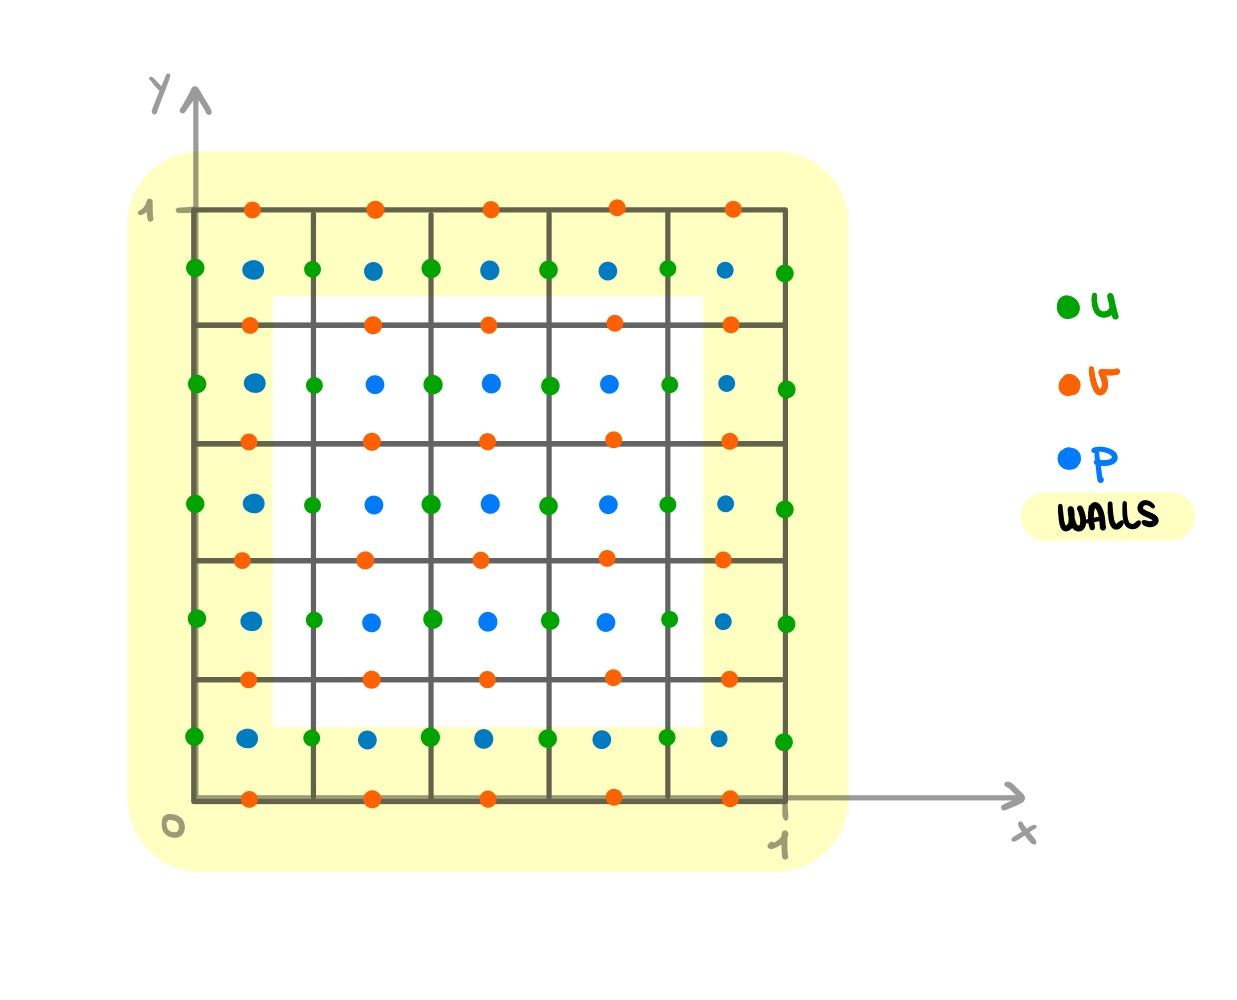
\includegraphics[width=0.5\textwidth]{discretization.jpg}
  \caption{Finite-volume discretization of the domain}
\end{figure}
The yellow line highlights the wall nodes, on which we are going to impose the following boundary conditions:
\begin{itemize}
    \item $v = 0$ on all the walls,
    \item $u = 1$ on the lid,
    \item $u = 0$ on the rest of the walls,
    \item $\frac{\partial p}{\partial n} = 0$ on all the walls.
\end{itemize}
With those boundary conditions we are able to enforce: the motion of the fluid in the proximity of the lid, the no-slip condition on the walls, and the zero-gradient normal condition for the pressure (impermeability of the walls).
In particular we can specify the boundary conditions for the pressure on the single walls as follows:
\begin{itemize}
    \item $\frac{\partial p}{\partial x} = 0$ on right and left walls,
    \item $\frac{\partial p}{\partial y} = 0$ on top and bottom walls.
\end{itemize}


\section*{\Large Task 3.1:}
To derive the finite-volume formulation of the problem, we first focus ont he x- momentum equation and perform the following steps, then we will do the same for the y-momentum equation. 
The starting point is the x-momentum equation:
\begin{equation}
    \frac{\partial u^2}{\partial x} + \frac{\partial uv}{\partial y} + \frac{\partial p}{\partial x} -\frac{1}{Re} (\frac{\partial^2 u}{\partial x^2} + \frac{\partial^2 u}{\partial y^2}) = 0
\end{equation}
We integrate over the control volume and we obtain:
\begin{equation}
    \int_{V} \frac{\partial}{\partial x} (u^2 - \frac{1}{Re} \frac{\partial u}{\partial x}) dV + \int_{V} \frac{\partial}{\partial y} (uv - \frac{1}{Re} \frac{\partial u}{\partial y}) + \int_{V} \frac{\partial p}{\partial x} dV = 0
\end{equation}
For simplicity we focus on the three integrals separately.

\subsubsection*{Discretization of the first convection-diffusion term}
We first apply the divergence theorem to the first term, in order to transform the volume integral into a surface integral, and then we split the integral over the whole surface into two contributions, one for the right surface and one for the left surface of the control volume:
\begin{equation} \label{discr_1}
  \int_{V} \frac{\partial}{\partial x} (u^2 - \frac{1}{Re} \frac{\partial u}{\partial x}) dV = \int_{S} (u^2 - \frac{1}{Re} \frac{\partial u}{\partial x}) \mathbf{n} dS = \int_{S_{i + \frac{1}{2}}} (u^2 - \frac{1}{Re} \frac{\partial u}{\partial x}) \mathbf{n} dS + \int_{S_{i - \frac{1}{2}}} (u^2 - \frac{1}{Re} \frac{\partial u}{\partial x}) \mathbf{n} dS
\end{equation}

Since the integrals are computed over the left and right surfaces of the control volume, we need to compute the velocities $u_{i + \frac{1}{2},j}$ and $u_{i - \frac{1}{2},j}$, which are not known since we store the velocity values at the faces of the control volumes. We can approximate these values by linear interpolation, as follows:
\begin{equation}
\begin{aligned}
  u_{i + \frac{1}{2},j} &= u_{i, j} + \frac{u_{i+1,j} - u_{i,j}}{\Delta x} \frac{\Delta x}{2} = 0.5 (u_{i,j} + u_{i+1,j})\\
  u_{i - \frac{1}{2},j} &= u_{i-1, j} + \frac{u_{i,j} - u_{i-1,j}}{\Delta x} \frac{\Delta x}{2} = 0.5 (u_{i-1,j} + u_{i,j})
\end{aligned}
\end{equation}

Then we compute the quadratic values as follows:
\begin{equation}
\begin{aligned}
  (u_{i + \frac{1}{2},j})^2 &=  0.25 (u_{i,j} + u_{i+1,j})^2\\
  (u_{i - \frac{1}{2},j})^2 &=  0.25 (u_{i-1,j} + u_{i,j})^2
\end{aligned}
\end{equation}

Now we can substitute the values of the velocities in \eqref{discr_1}:
\begin{flalign}
  & \int_{S_{i + \frac{1}{2}}} \left(u^2 - \frac{1}{Re} \frac{\partial u}{\partial x}\right) \mathbf{n} dS + \int_{S_{i - \frac{1}{2}}} \left(u^2 - \frac{1}{Re} \frac{\partial u}{\partial x}\right) \mathbf{n} dS = \notag \\
  & \left(0.25 (u_{i,j} + u_{i+1,j})^2 - \frac{1}{Re} \left(\frac{u_{i+1,j} - u_{i,j}}{\Delta x}\right)\right) \Delta y - \left(0.25 (u_{i-1,j} + u_{i,j})^2 - \frac{1}{Re} \left(\frac{u_{i,j} - u_{i-1,j}}{\Delta x}\right)\right) \Delta y
  \end{flalign}
where the minus sign in front of the second term is due to the fact that the normal vector is pointing in the opposite direction with respect to the first term.

As last step we need to perform linearization since we have quadratic terms in the expression. To perform the linearization we use the formulation $ u^2 = u u \approx u^* u$ where $u^*$ is a previously computed value of the velocity (e.g. the value at the previous iteration of the initial guess). It is important to notice that $u^*$ is not the value of the velocity at the preious time step since we are in a time independent formulation.
This leads us to the following expression:
\begin{equation}
  \begin{aligned}
  0.25 (u_{i,j} + u_{i+1,j})^2 \approx 0.25 (u^*_{i,j} + u^*_{i+1,j}) (u_{i,j} + u_{i+1,j}) &= 0.25 (u^*_{i,j} u_{i,j} + u^*_{i+1,j} u_{i+1,j} + u^*_{i,j} u_{i+1,j} + u^*_{i+1,j} u_{i,j}) \\
  0.25 (u_{i-1,j} + u_{i,j})^2 \approx 0.25 (u^*_{i-1,j} + u^*_{i,j}) (u_{i-1,j} + u_{i,j}) &= 0.25 (u^*_{i-1,j} u_{i-1,j} + u^*_{i,j} u_{i,j} + u^*_{i-1,j} u_{i,j} + u^*_{i,j} u_{i-1,j})
  \end{aligned}
\end{equation}

Including the linearization in the discretization we obtain:
\begin{flalign}
  & \int_{V} \frac{\partial}{\partial x} (u^2 - \frac{1}{Re} \frac{\partial u}{\partial x}) dV \approx \notag \\
  & \left(0.25 (u^*_{i,j} u_{i,j} + u^*_{i+1,j} u_{i+1,j} + u^*_{i,j} u_{i+1,j} + u^*_{i+1,j} u_{i,j}) - \frac{1}{Re} \frac{u_{i+1,j} - u_{i,j}}{\Delta x}\right) \Delta y \notag \\
  & - \left(0.25 (u^*_{i-1,j} u_{i-1,j} + u^*_{i,j} u_{i,j} + u^*_{i-1,j} u_{i,j} + u^*_{i,j} u_{i-1,j}) - \frac{1}{Re} \frac{u_{i,j} - u_{i-1,j}}{\Delta x}\right) \Delta y
\end{flalign}

\subsubsection*{Discretization of the second convection-diffusion term}
For the second term we proceed in the same way as before and we obtain:
\begin{flalign} \label{discr_2}
  & \int_{V} \frac{\partial}{\partial y} (uv - \frac{1}{Re} \frac{\partial u}{\partial y}) dV = \int_{S} (uv - \frac{1}{Re} \frac{\partial u}{\partial y}) \mathbf{n} dS = \int_{S_{j + \frac{1}{2}}} (uv - \frac{1}{Re} \frac{\partial u}{\partial y}) \mathbf{n} dS + \int_{S_{j - \frac{1}{2}}} (uv - \frac{1}{Re} \frac{\partial u}{\partial y}) \mathbf{n} dS = \notag \\
  & \left(0.25 (u_{i,j} + u_{i,j+1}) (v_{i,j} + v_{i+1,j}) - \frac{1}{Re} \frac{u_{i,j+1} - u_{i,j}}{\Delta y}\right) \Delta x - \left(0.25 (u_{i,j-1} + u_{i,j}) (v_{i,j-1} + v_{i+1,j-1}) - \frac{1}{Re} \frac{u_{i,j} - u_{i,j-1}}{\Delta y}\right) \Delta x
\end{flalign}
It is important to notice that now $S_{j + \frac{1}{2}}$ and $S_{j - \frac{1}{2}}$ are the surfaces on the top and bottom of the control volume. 

At this point we need to perform the linearization due to the product between the velocities, but this time we can not use the same formulation as before since the term is not a quadratic term. We can use the following formulation: $ uv \approx u^* v + u v^* - u^* v^*$.
This allows us to transform the $uv$ terms as follows
\begin{equation}
\begin{aligned}
  (u_{i,j} + u_{i,j+1}) (v_{i,j} + v_{i+1,j}) &\approx (u^*_{i,j} + u^*_{i,j+1}) (v_{i,j} + v_{i+1,j}) +(u_{i,j} + u_{i,j+1}) (v^*_{i,j} + v^*_{i+1,j}) - (u^*_{i,j} + u^*_{i,j+1}) (v^*_{i,j} + v^*_{i+1,j}) \\
  & = u^*_{i,j}v_{i,j} + u^*_{i,j}v_{i+1,j} + u^*_{i,j+1}v_{i,j} + u^*_{i,j+1}v_{i+1,j} \\
  & + u_{i,j}v^*_{i,j} + u_{i,j+1}v^*_{i,j} + u_{i,j}v^*_{i+1,j} + u_{i,j+1}v^*_{i+1,j} \\
  & - (u^*_{i,j} + u^*_{i,j+1}) (v^*_{i,j} + v^*_{i+1,j}) \\
  (u_{i,j-1} + u_{i,j}) (v_{i,j-1} + v_{i+1,j-1}) &\approx (u^*_{i,j-1} + u^*_{i,j}) (v_{i,j-1} + v_{i+1,j-1}) + (u_{i,j-1} + u_{i,j}) (v^*_{i,j-1} + v^*_{i+1,j-1})\\
  &- (u^*_{i,j-1} + u^*_{i,j}) (v^*_{i,j-1} + v^*_{i+1,j-1}) \\
  & = u^*_{i,j-1}v_{i,j-1} + u^*_{i,j-1}v_{i+1,j-1} + u^*_{i,j}v_{i,j-1} + u^*_{i,j}v_{i+1,j-1} \\
  & + u_{i,j-1}v^*_{i,j-1} + u_{i,j}v^*_{i,j-1} + u_{i,j-1}v^*_{i+1,j-1} + u_{i,j}v^*_{i+1,j-1} \\
  & - (u^*_{i,j-1} + u^*_{i,j}) (v^*_{i,j-1} + v^*_{i+1,j-1})
\end{aligned}
\end{equation}

Substituting the linearized terms in the discretization \eqref{discr_2} we obtain:
\begin{equation}
  \begin{aligned}
  \int_{V} \frac{\partial}{\partial y} (uv - \frac{1}{Re} \frac{\partial u}{\partial y}) dV = & (0.25 (u^*_{i,j}v_{i,j} + u^*_{i,j}v_{i+1,j} + u^*_{i,j+1}v_{i,j} + u^*_{i,j+1}v_{i+1,j} \\
  & + u_{i,j}v^*_{i,j} + u_{i,j+1}v^*_{i,j} + u_{i,j}v^*_{i+1,j} + u_{i,j+1}v^*_{i+1,j} \\
  & - (u^*_{i,j} + u^*_{i,j+1}) (v^*_{i,j} + v^*_{i+1,j})) - \frac{1}{Re} \frac{u_{i,j+1} - u_{i,j}}{\Delta y}) \Delta x \\
  & - (0.25 (u^*_{i,j-1}v_{i,j-1} + u^*_{i,j-1}v_{i+1,j-1} + u^*_{i,j}v_{i,j-1} + u^*_{i,j}v_{i+1,j-1} \\
  & + u_{i,j-1}v^*_{i,j-1} + u_{i,j}v^*_{i,j-1} + u_{i,j-1}v^*_{i+1,j-1} + u_{i,j}v^*_{i+1,j-1} \\
  & - (u^*_{i,j-1} + u^*_{i,j}) (v^*_{i,j-1} + v^*_{i+1,j-1})) - \frac{1}{Re} \frac{u_{i,j} - u_{i,j-1}}{\Delta y}) \Delta x
  \end{aligned}
\end{equation}


\subsubsection*{Discretization of the pressure term}
Since we don't know the pressure distribution inside the control volumes, we need to perform an approxiamtion taking into account that we only know the pressure values at the cell centers.
\begin{equation}
\begin{aligned}
  \int_{V} \frac{\partial p}{\partial x} dV &= \overline{\frac{\partial p}{\partial x}} \Delta V 
  \approx \frac{\partial p}{\partial x} \Delta V 
  = \frac{p_{i+1,j} - p_{i,j}}{\Delta x} \Delta x \Delta y 
  = \Delta y (p_{i+1,j} - p_{i,j})
\end{aligned}
\end{equation}
First we assume that the pressure gradient is constant inside the control volume, then we approximate $\frac{\partial p}{\partial x}$ as the difference between the pressure at the cell center on the right and the pressure at the cell center on the cell we are considering. We multiply this difference by the volume of the control volume to obtain the integral.


\subsubsection*{Complete discretization of the momentum equations}
Now we assemble the complete discretization by combining the three terms:
\begin{equation}
  \begin{aligned}
    & (0.25 (u^*_{i,j} u_{i,j} + u^*_{i+1,j} u_{i+1,j} + u^*_{i,j} u_{i+1,j} + u^*_{i+1,j} u_{i,j}) - \frac{1}{Re} \frac{u_{i+1,j} - u_{i,j}}{\Delta x}) \Delta y  \\
    & - (0.25 (u^*_{i-1,j} u_{i-1,j} + u^*_{i,j} u_{i,j} + u^*_{i-1,j} u_{i,j} + u^*_{i,j} u_{i-1,j}) - \frac{1}{Re} \frac{u_{i,j} - u_{i-1,j}}{\Delta x}) \Delta y \\
    & + (0.25 (u^*_{i,j}v_{i,j} + u^*_{i,j}v_{i+1,j} + u^*_{i,j+1}v_{i,j} + u^*_{i,j+1}v_{i+1,j} \\
    & + u_{i,j}v^*_{i,j} + u_{i,j+1}v^*_{i,j} + u_{i,j}v^*_{i+1,j} + u_{i,j+1}v^*_{i+1,j} \\
    & - (u^*_{i,j} + u^*_{i,j+1}) (v^*_{i,j} + v^*_{i+1,j})) - \frac{1}{Re} \frac{u_{i,j+1} - u_{i,j}}{\Delta y}) \Delta x \\
    & - (0.25 (u^*_{i,j-1}v_{i,j-1} + u^*_{i,j-1}v_{i+1,j-1} + u^*_{i,j}v_{i,j-1} + u^*_{i,j}v_{i+1,j-1} \\
    & + u_{i,j-1}v^*_{i,j-1} + u_{i,j}v^*_{i,j-1} + u_{i,j-1}v^*_{i+1,j-1} + u_{i,j}v^*_{i+1,j-1} \\
    & - (u^*_{i,j-1} + u^*_{i,j}) (v^*_{i,j-1} + v^*_{i+1,j-1})) - \frac{1}{Re} \frac{u_{i,j} - u_{i,j-1}}{\Delta y}) \Delta x \\
    & + \Delta y (p_{i+1,j} - p_{i,j}) = 0
  \end{aligned}
\end{equation}

The finite-volume formulation of the $x$-momentum equation consists in a balancing of the forces acting on a control volume.
Convective terms, which are in the form $u*u$, represent momentum transport due to fluid motion and are evaluated at control volume vertical faces using linear interpolation and linearization.
Diffusion terms, which are the ones like $-\frac{1}{Re} \frac{u_{i+1,j} - u_{i,j}}{\Delta x}$, account for viscous effects, with velocity gradients calculated at the horizontal faces.
Cross-convection terms, which consist in the multiplication between $v$ and $u$, capture the interaction between $x$- and $y$- velocity components, while the pressure gradient term drives flow and is determined using interpolated cell-center values.

The discretization of the y-momentum equation can be obtained following an analogous procedure, where $x$ and $y$, and $u$ and $v$ are swapped in the equations, and in the end we obtain the following expression:
\begin{equation}
  \begin{aligned}
    & (0.25 (v^*_{i,j} v_{i,j} + v^*_{i,j+1} v_{i,j+1} + v^*_{i,j} v_{i,j+1} + v^*_{i,j+1} v_{i,j}) - \frac{1}{Re} \frac{v_{i,j+1} - v_{i,j}}{\Delta y}) \Delta x  \\
    & - (0.25 (v^*_{i,j-1} v_{i,j-1} + v^*_{i,j} v_{i,j} + v^*_{i,j-1} v_{i,j} + v^*_{i,j} v_{i,j-1}) - \frac{1}{Re} \frac{v_{i,j} - v_{i,j-1}}{\Delta y}) \Delta x \\
    & + (0.25 (v^*_{i,j}u_{i,j} + v^*_{i,j}u_{i+1,j} + v^*_{i+1,j}u_{i,j} + v^*_{i+1,j}u_{i+1,j} \\
    & + v_{i,j}u^*_{i,j} + v_{i,j}u^*_{i+1,j} + v_{i+1,j}u^*_{i,j} + v_{i+1,j}u^*_{i+1,j} \\
    & - (v^*_{i,j} + v^*_{i+1,j}) (u^*_{i,j} + u^*_{i+1,j})) - \frac{1}{Re} \frac{v_{i+1,j} - v_{i,j}}{\Delta x}) \Delta y \\
    & - (0.25 (v^*_{i-1,j}u_{i-1,j} + v^*_{i-1,j}u_{i,j} + v^*_{i,j}u_{i-1,j} + v^*_{i,j}u_{i,j} \\
    & + v_{i-1,j}u^*_{i-1,j} + v_{i-1,j}u^*_{i,j} + v_{i,j}u^*_{i-1,j} + v_{i,j}u^*_{i,j} \\
    & - (v^*_{i-1,j} + v^*_{i,j}) (u^*_{i-1,j} + u^*_{i,j})) - \frac{1}{Re} \frac{v_{i,j} - v_{i-1,j}}{\Delta x}) \Delta y \\
    & + \Delta x (p_{i,j+1} - p_{i,j}) = 0
  \end{aligned}
\end{equation}

In the picture reported below we can see which are the reference control volumes for each of the three equations, moreover we can see
that the center of each control volume is the point where we store the variable ($u$, $v$ and $p$) we are computing in this specific control volume with the corresponding equation.

\begin{figure}[h!]
  \centering
  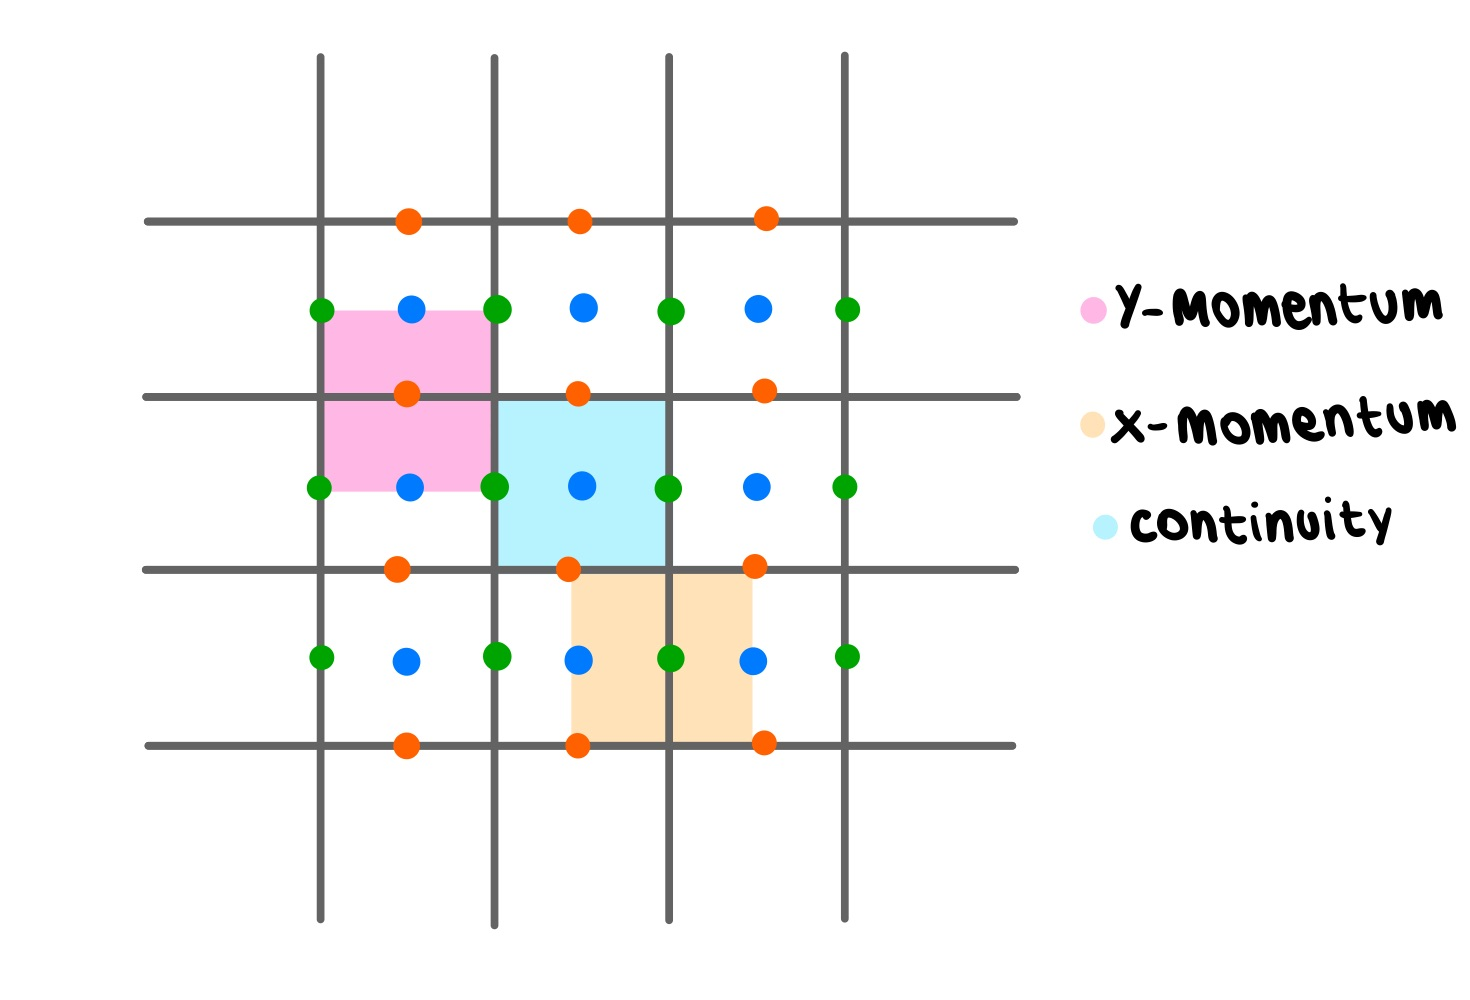
\includegraphics[width=0.5\textwidth]{controlvolumes.jpg}
  \caption{Control volumes}
\end{figure}


\section*{\Large Task 3.2:}
\section*{\Large Task 3.3:}
\section*{\Large Task 3.4:}
\section*{\Large Task 3.5:}
\section*{\Large Task 3.6:}
\section*{\Large Task 3.7:}

\begin{thebibliography}{9}
    \bibitem{GitHubRepo}
    \textit{CFD Repository},\\
    Available at: \url{https://github.com/GiuseppePisante/CFD.git}
    
    \bibitem{GitHubCopilot}
    \textit{GitHub Copilot},\\
    GitHub. Available at: \url{https://github.com/features/copilot}
    \end{thebibliography}

\end{document}